%!TEX root = ../thesis.tex
\chapter{Results}
\label{ch:results}

\begin{itemize}
    \item Gleitenden Mittelwert bei Darstellung mit Window Size 20 um das Grundrauschen zu minimieren
\end{itemize}
\section{Oriented Bounding Boxes and Axis Aligned Bounding Boxes}
\begin{itemize}
    \item obb weil performance bei Map40-95 in allen Epochen besser
    \item Map bei obb zwiscehn 0.5 und 0.6; bei abb bei 0.35 und 0.45
    \item Bei gleichen Bounding box koordinaten ist obb bei 0.55 und 0.59 und abb 0.59 und 0.6
    \item bessere Performance von abb wahrscheinlich weil geringe Änderungen in der Orientierung der Bounding Boxen eine hohe Auswirkung auf die Genauigkeit der Boxen haben
\end{itemize}

\section{RGBIR vs. ... (map5-95)}

\begin{figure}[h] 
    \centering % Centers the graphic horizontally
    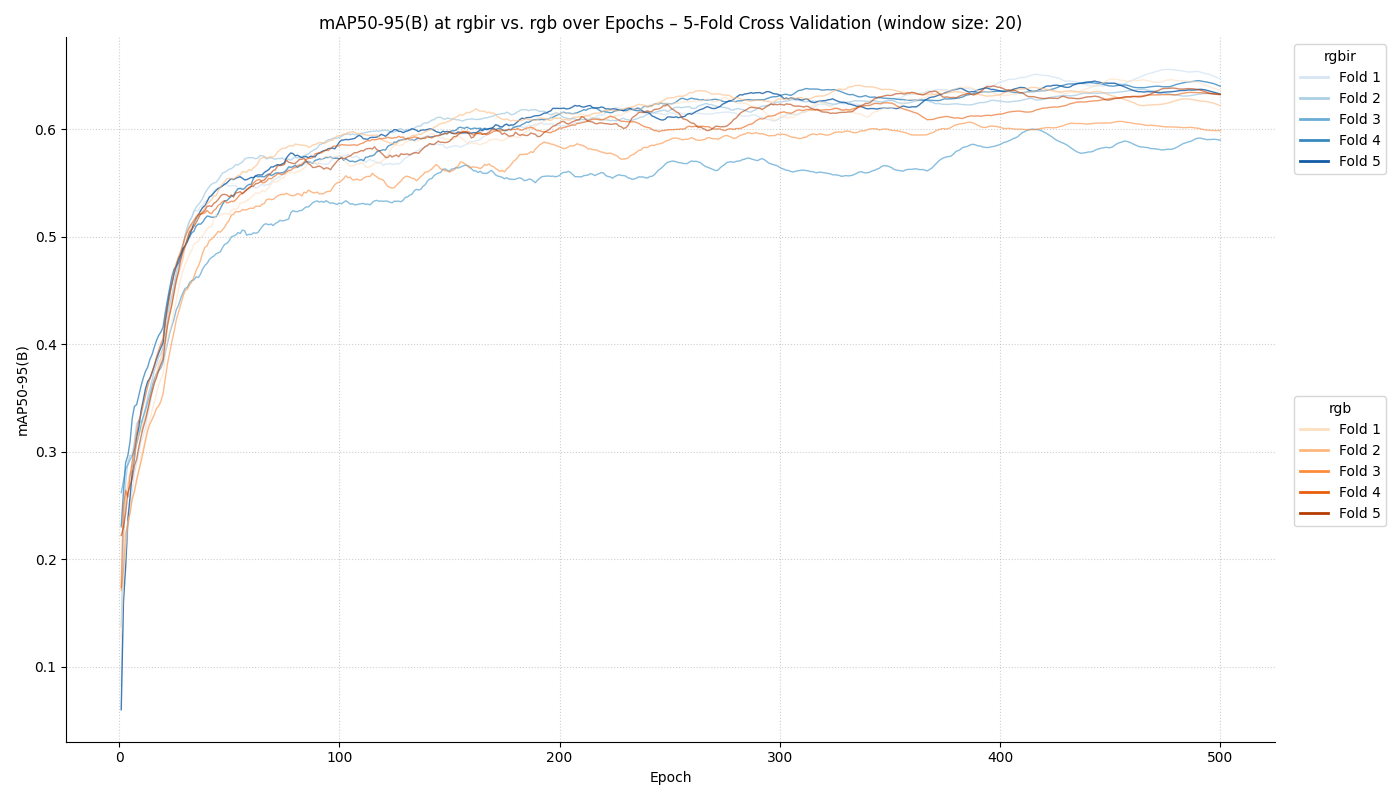
\includegraphics[width=1\textwidth]{images/rgbir/mAP@50-95/rgbir_vs_rgb_full.png} % Path to the graphic file
    \caption{Comparison of mAP50(B) over 200 Epochs for rgbir vs. rgb.} % Image caption
    \label{fig:map_rgir_rgb} % Label for references in the text
\end{figure}
\begin{itemize}
    \item Insgesamt ist ein ansteigender Trend über alle Epochen hinweg zu beobachten. Der Anstieg der Leistung ist in den Anfangsepochen signifikanter und flacht dann ab, um im weiteren Verlauf bis Epoche 500 zu konvergieren.
    \item RGB IR hat bessere Spitzenleistung als RGB.  
    \item RGBIR erreicht konsequent höhere absolute mAP-Werte 
    \item Über die längere Trainingsdauer verfestigt sich der anfängliche Vorteil von RGBIR. Die RGB Modelle liegen bei einer mAP von 0.60-0.62, während die besten RGBIR Modelle Werte um 0.62-0.65 mAP erreichen.
    \item Ab Epoche 300-400 erreichen beide Modelle ein Plateu, ab dem die Leistung nur noch geringfügig schwankt, was darauf hindeutet, dass die Modelle weitgehend konvergiert sind.
\end{itemize}



\begin{itemize}
    \item Signifikant schlechtere map bei Modellen mit NDVI Kanal im Datensatz, unabhängig von Kanalanzahl (RGB NDVI und GB NDVI)
    \item RGB: Performance relativ ähnlich, alles wenig schwankungen. Zusätzlicher kanal hat wenig auswirkugnen
\end{itemize}

\begin{figure}[h] 
    \centering
    % Erste Subfigur
    \begin{subfigure}[b]{0.85\textwidth} % [b] für bottom alignment, 0.48\textwidth damit noch Platz ist
        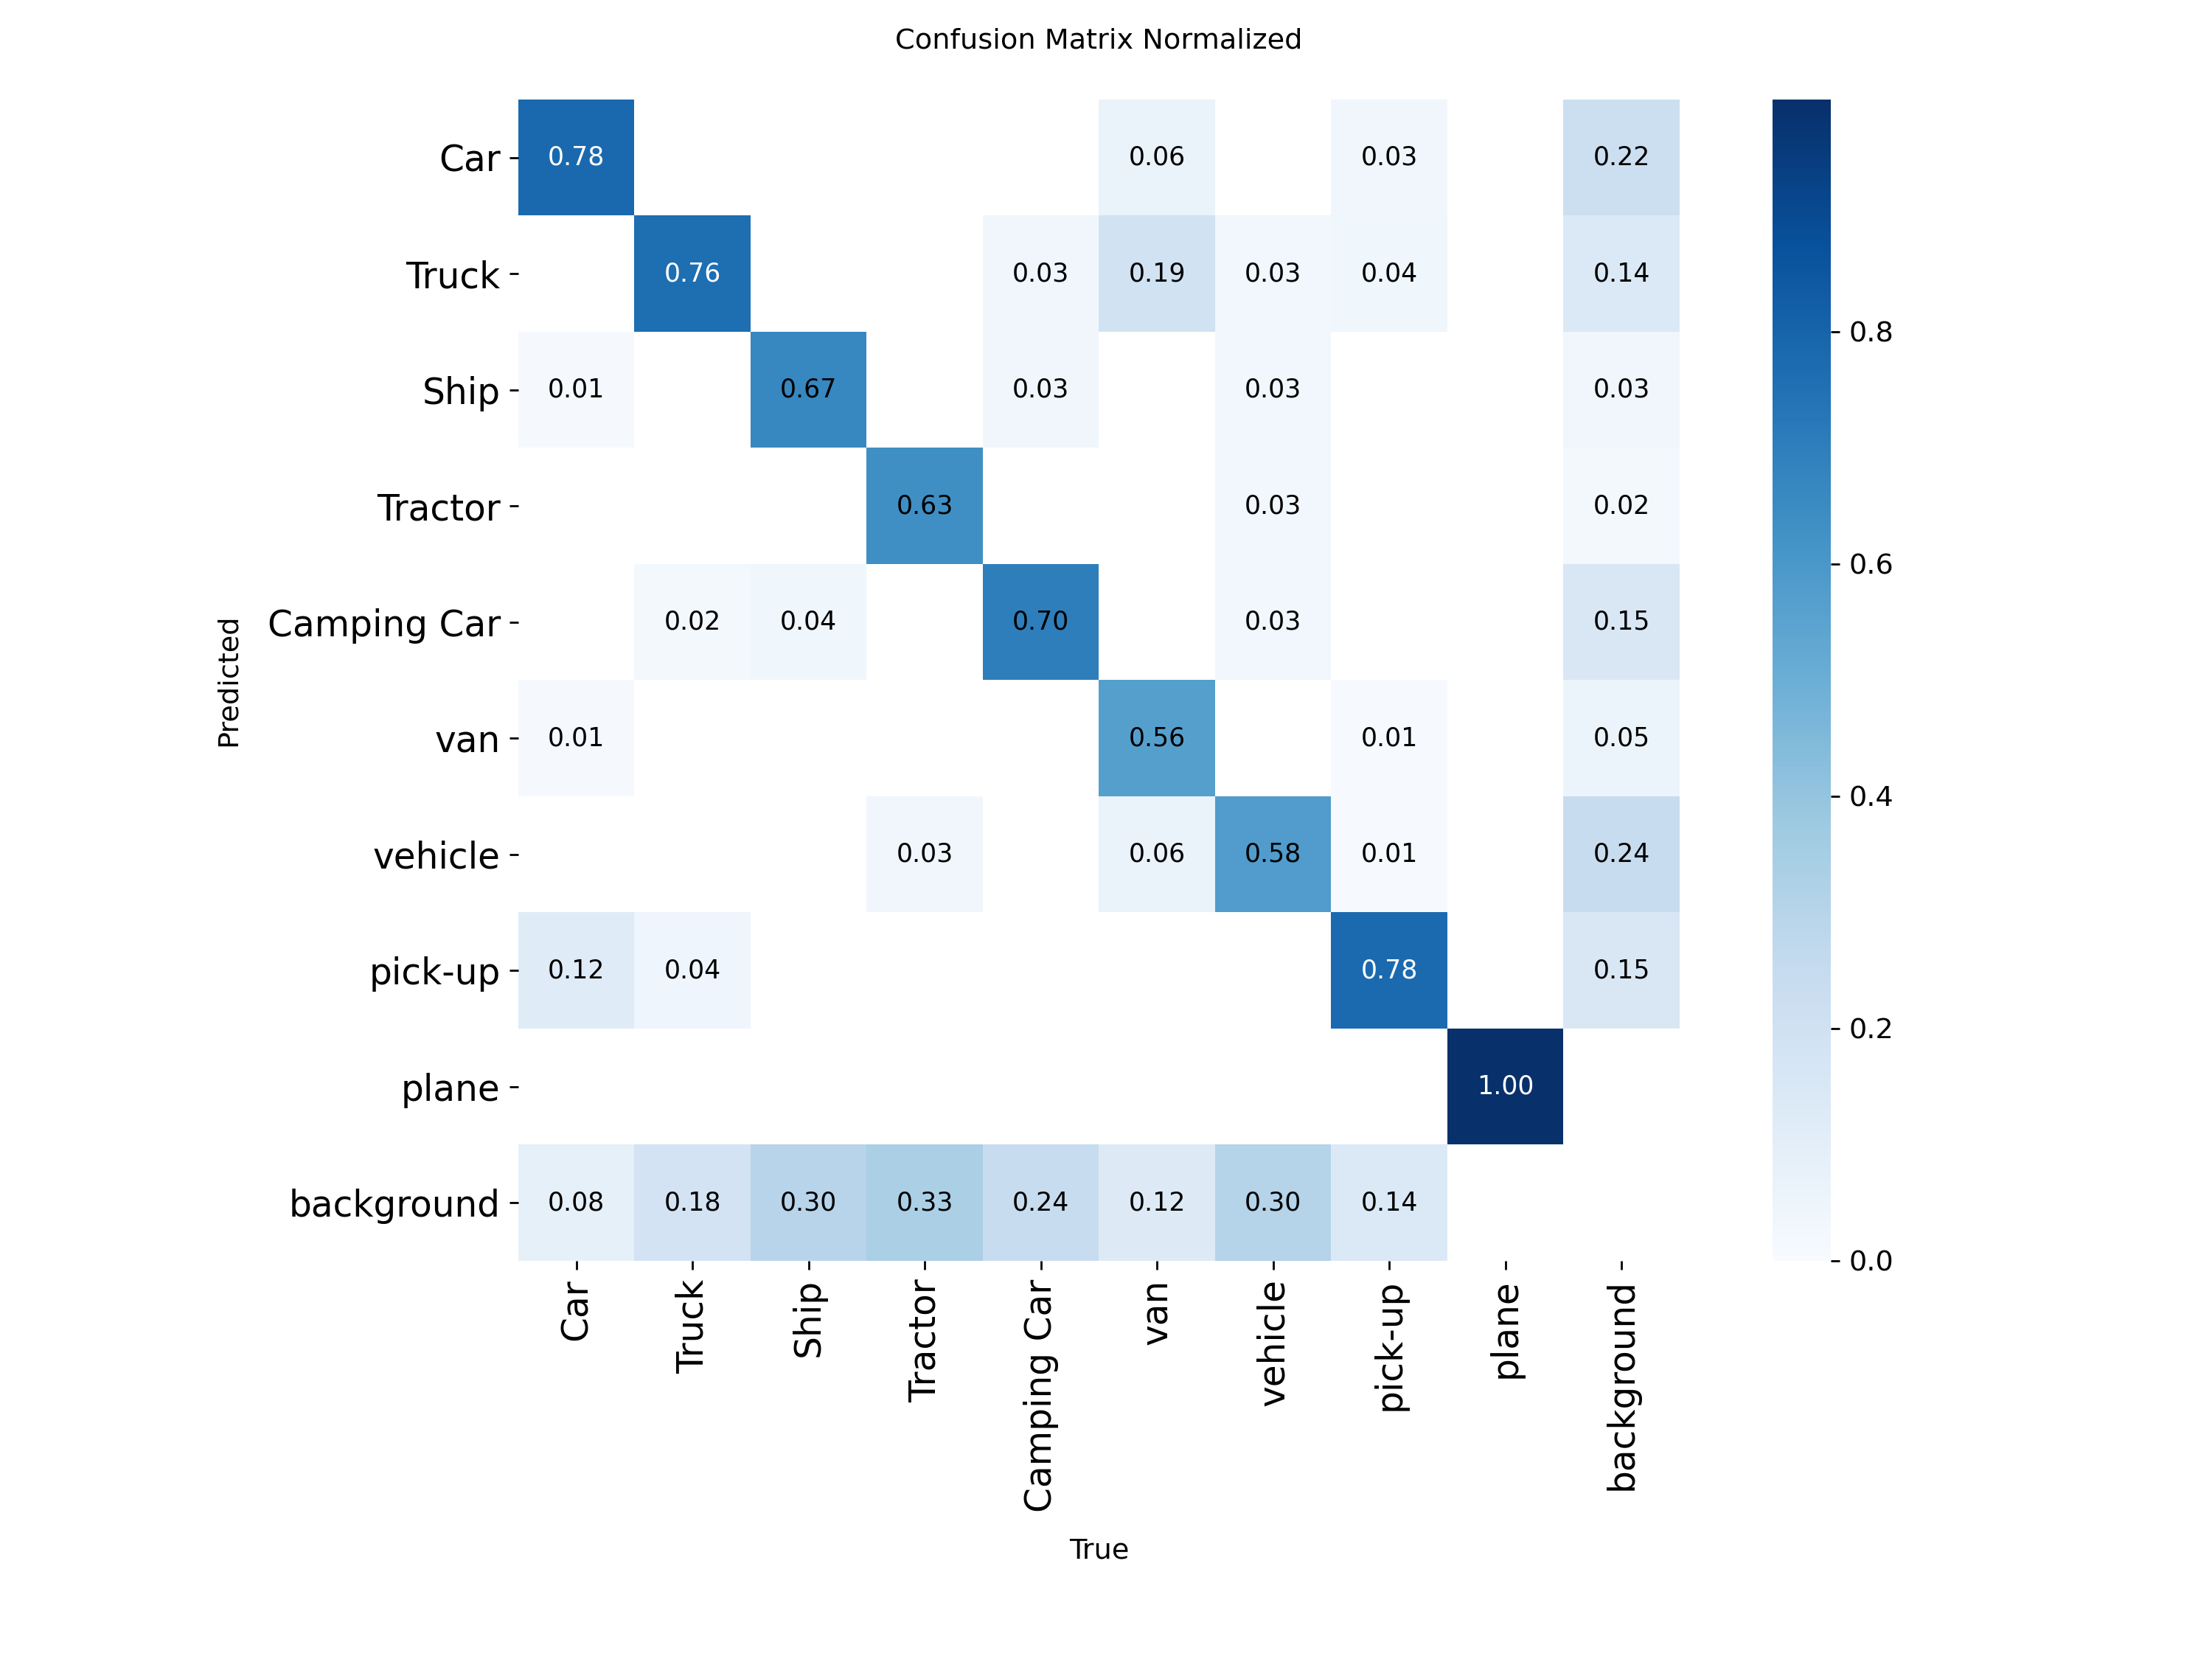
\includegraphics[width=\textwidth]{images/confusion_matrices/rgbir_F4_confusion_matrix_normalized.png} % Bildpfad zum ersten Bild
        \caption{r-g-b-ir} % Unterschrift für das erste Bild
        \label{fig:cm_trgbir} % Label für Referenzierung von Bild 1
    \end{subfigure}
    \hfill % Fügt horizontalen Platz zwischen den Subfiguren ein
    % Zweite Subfigur
    \begin{subfigure}[b]{0.85\textwidth} % 0.48\textwidth für das zweite Bild
        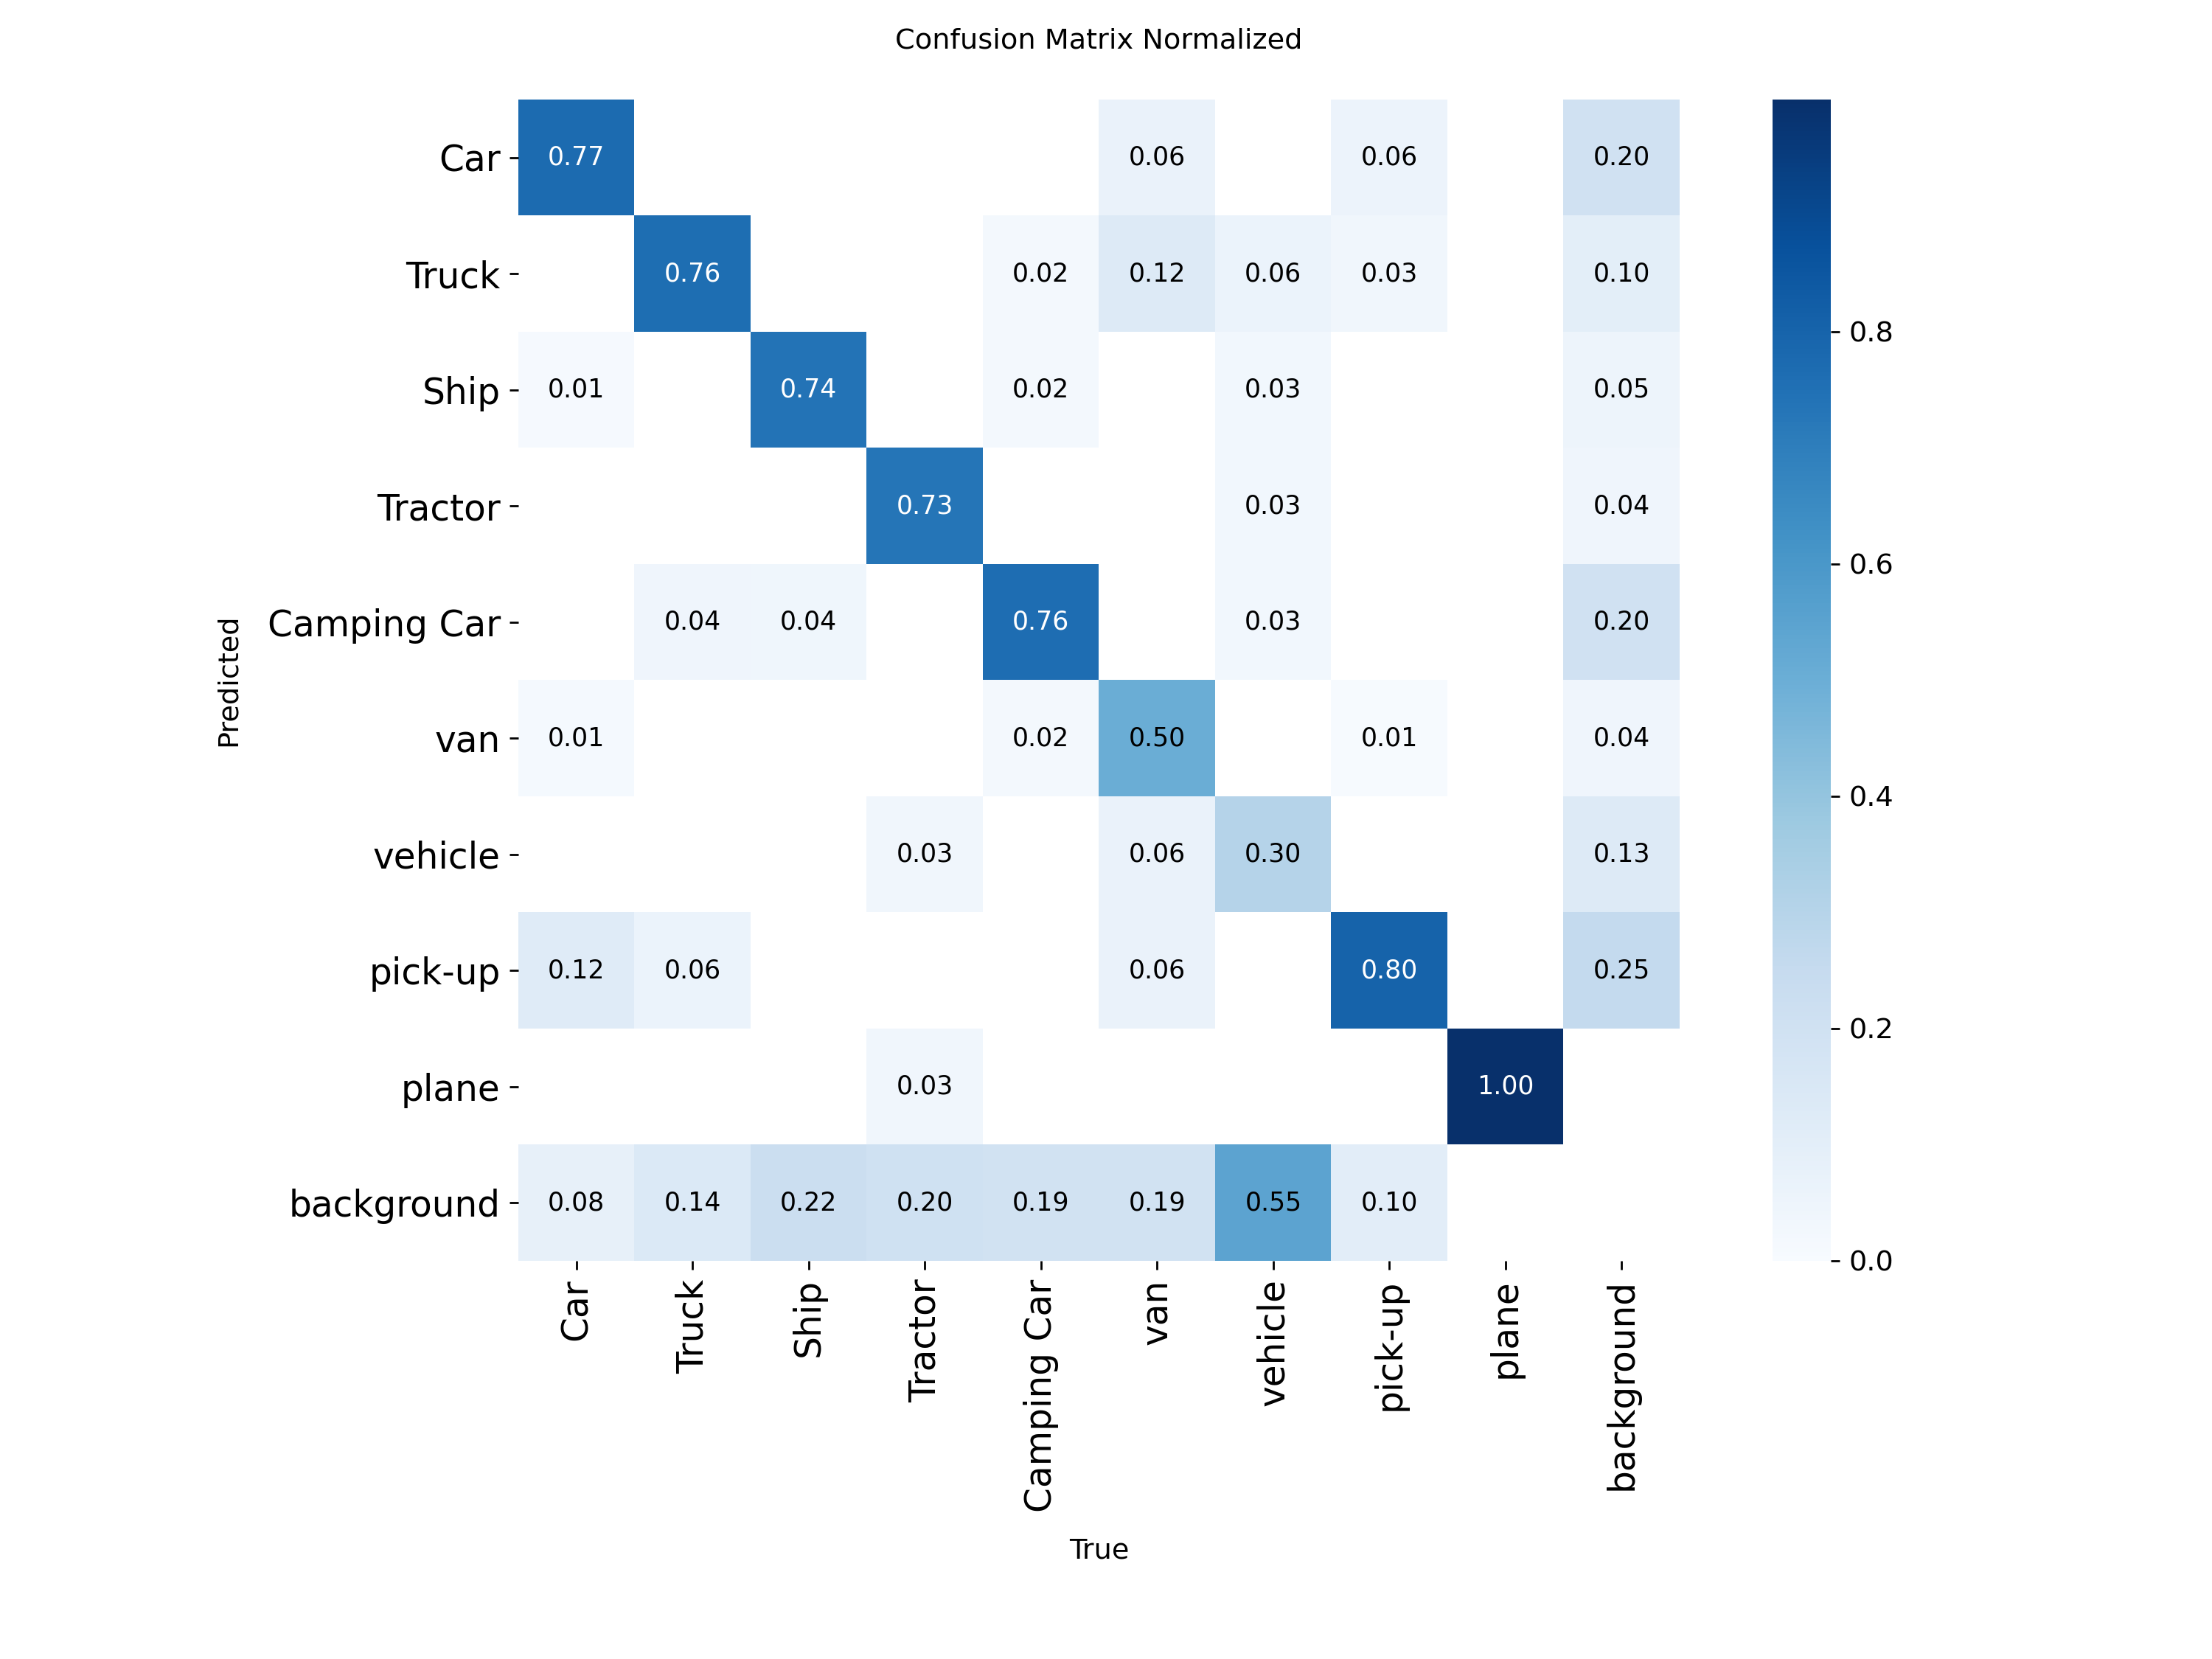
\includegraphics[width=\textwidth]{images/confusion_matrices/irgb_F4_confusion_matrix_normalized.png} % Bildpfad zum zweiten Bild
        \caption{ir-g-b} % Unterschrift für das zweite Bild
        \label{fig:cm_irgb} % Label für Referenzierung von Bild 2
    \end{subfigure}
    \caption{Comparison of Confusion Matrices between r-g-b-ir und ir-g-b for Fold 4} % Gemeinsame Unterschrift für beide Bilder
    \label{fig:combined_maps} % Label für die gesamte Figure-Umgebung
\end{figure}

\begin{figure}[h] 
    \centering
    % Erste Subfigur
    \begin{subfigure}[b]{0.85\textwidth} % [b] für bottom alignment, 0.48\textwidth damit noch Platz ist
        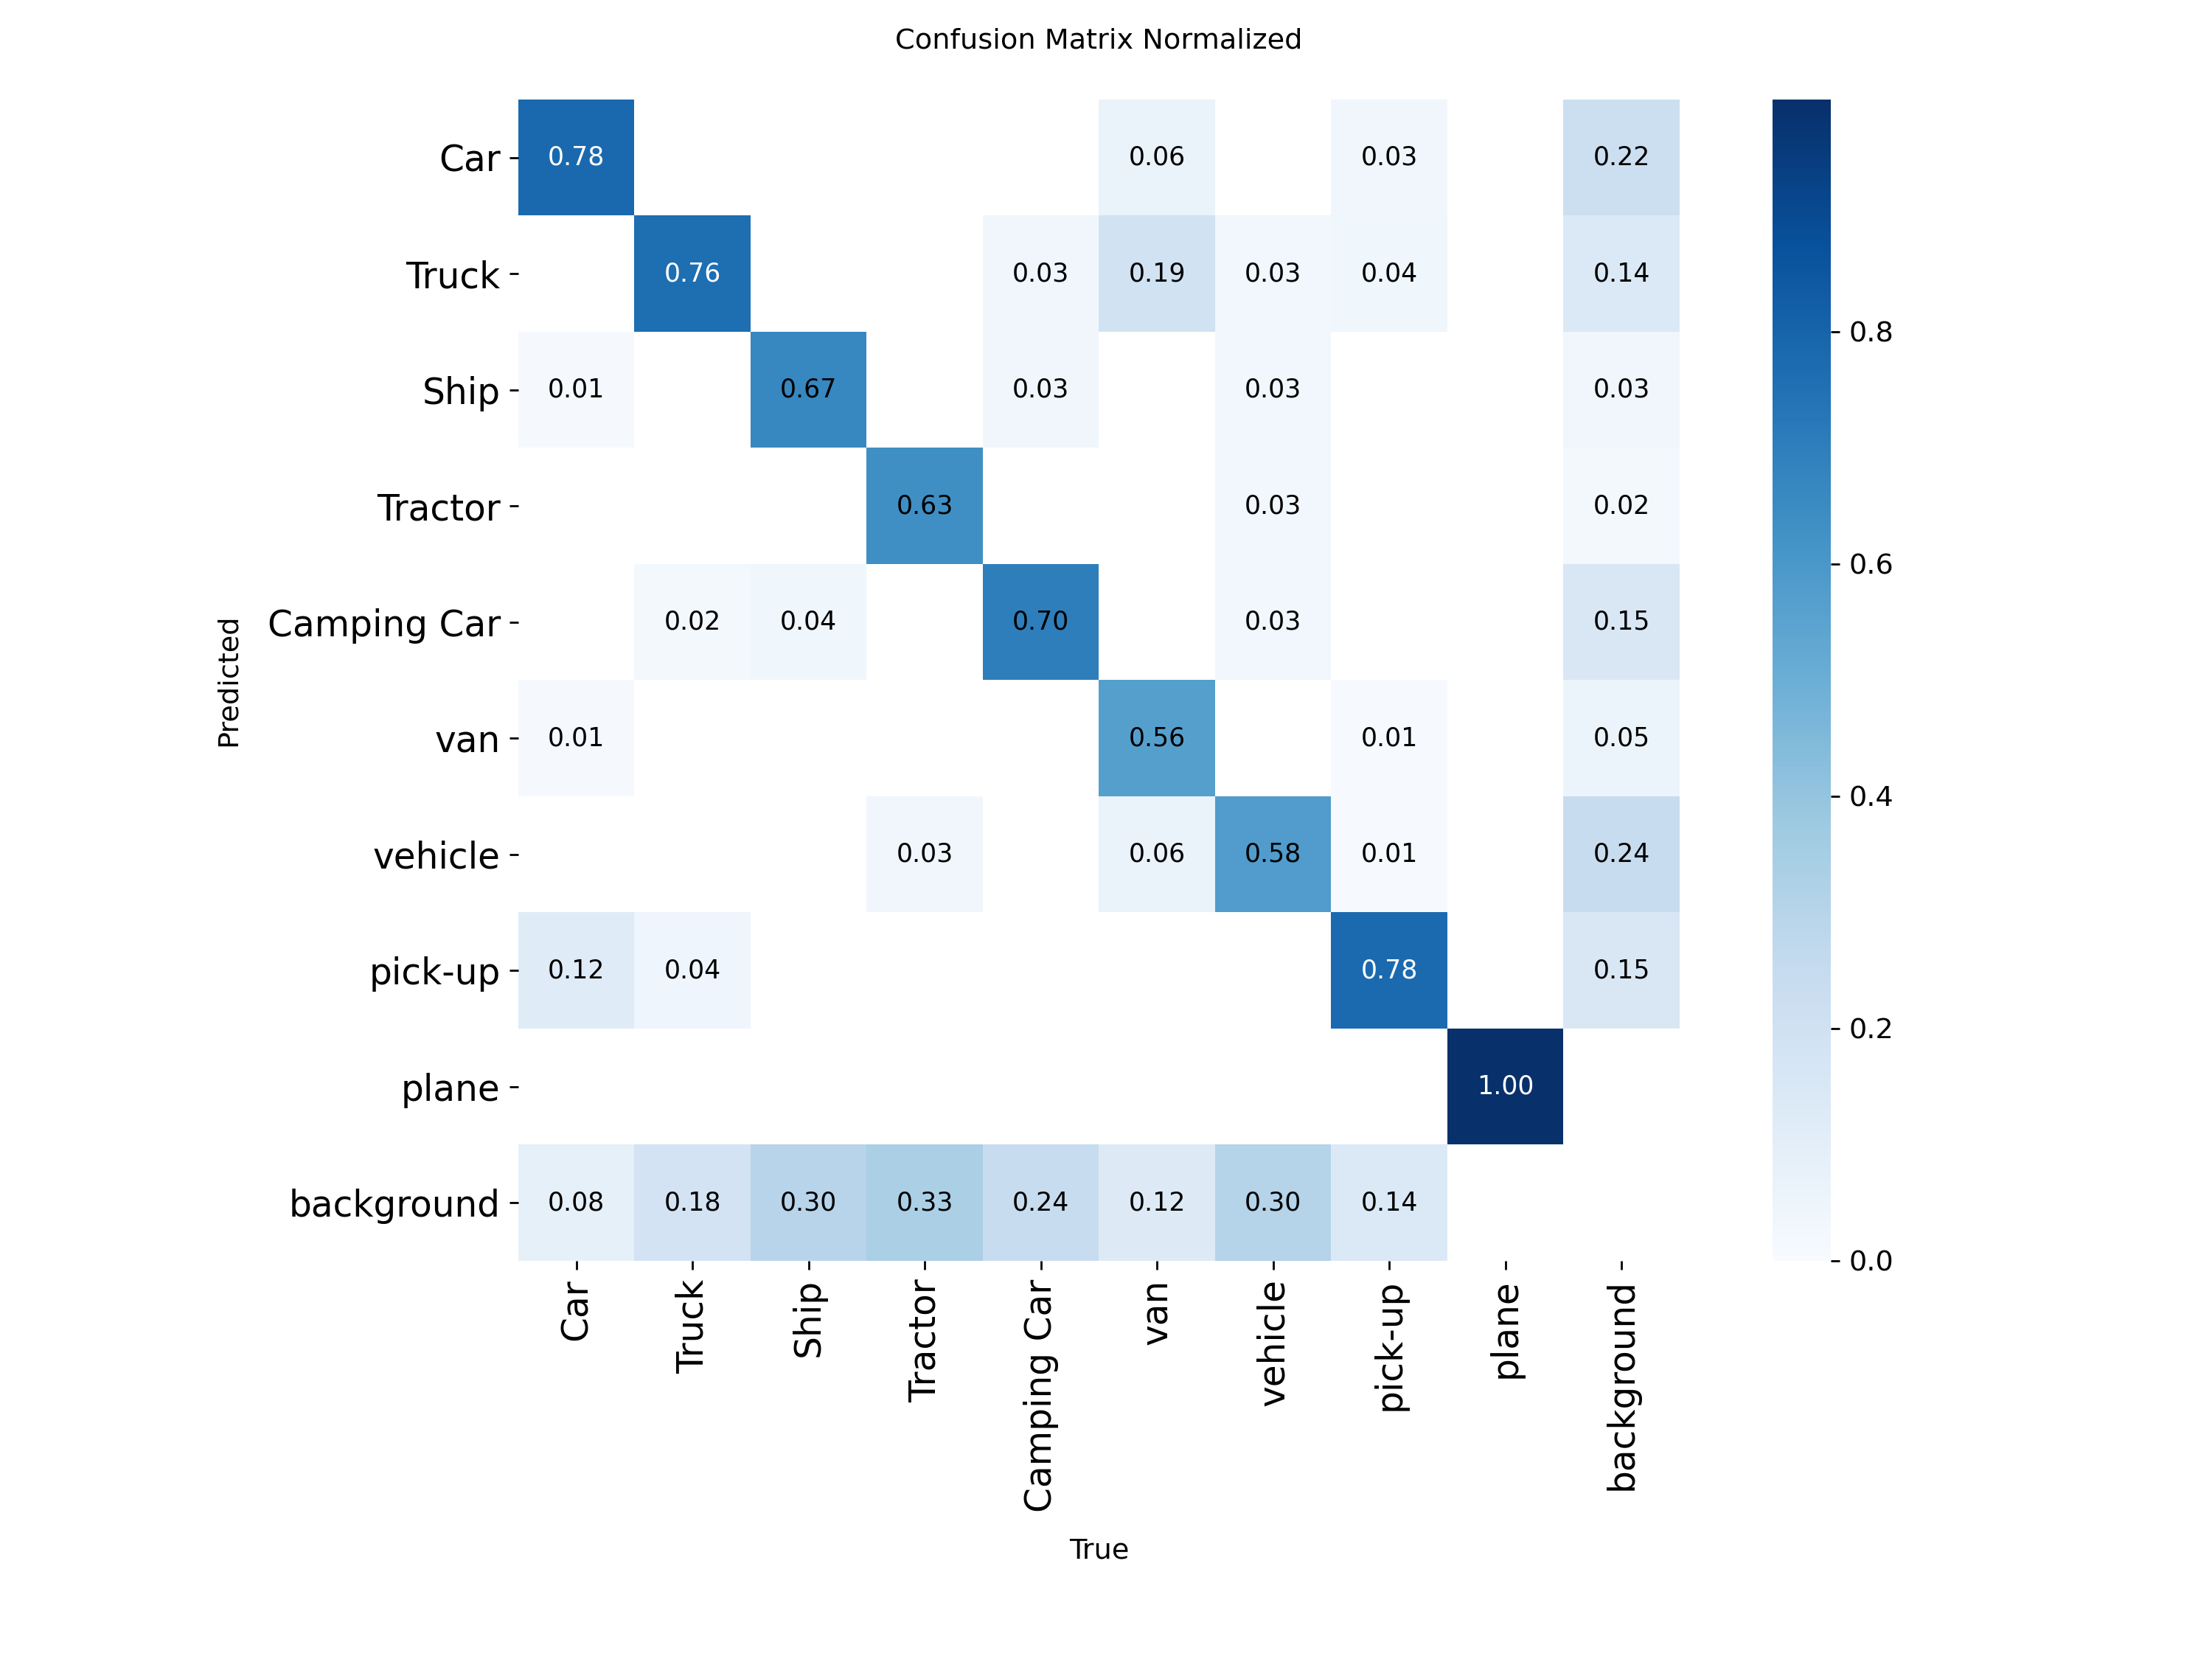
\includegraphics[width=\textwidth]{images/confusion_matrices/rgbir_F4_confusion_matrix_normalized.png} % Bildpfad zum ersten Bild
        \caption{r-g-b-ir} % Unterschrift für das erste Bild
        \label{fig:cm_trgbir} % Label für Referenzierung von Bild 1
    \end{subfigure}
    \hfill % Fügt horizontalen Platz zwischen den Subfiguren ein
    % Zweite Subfigur
    \begin{subfigure}[b]{0.85\textwidth} % 0.48\textwidth für das zweite Bild
        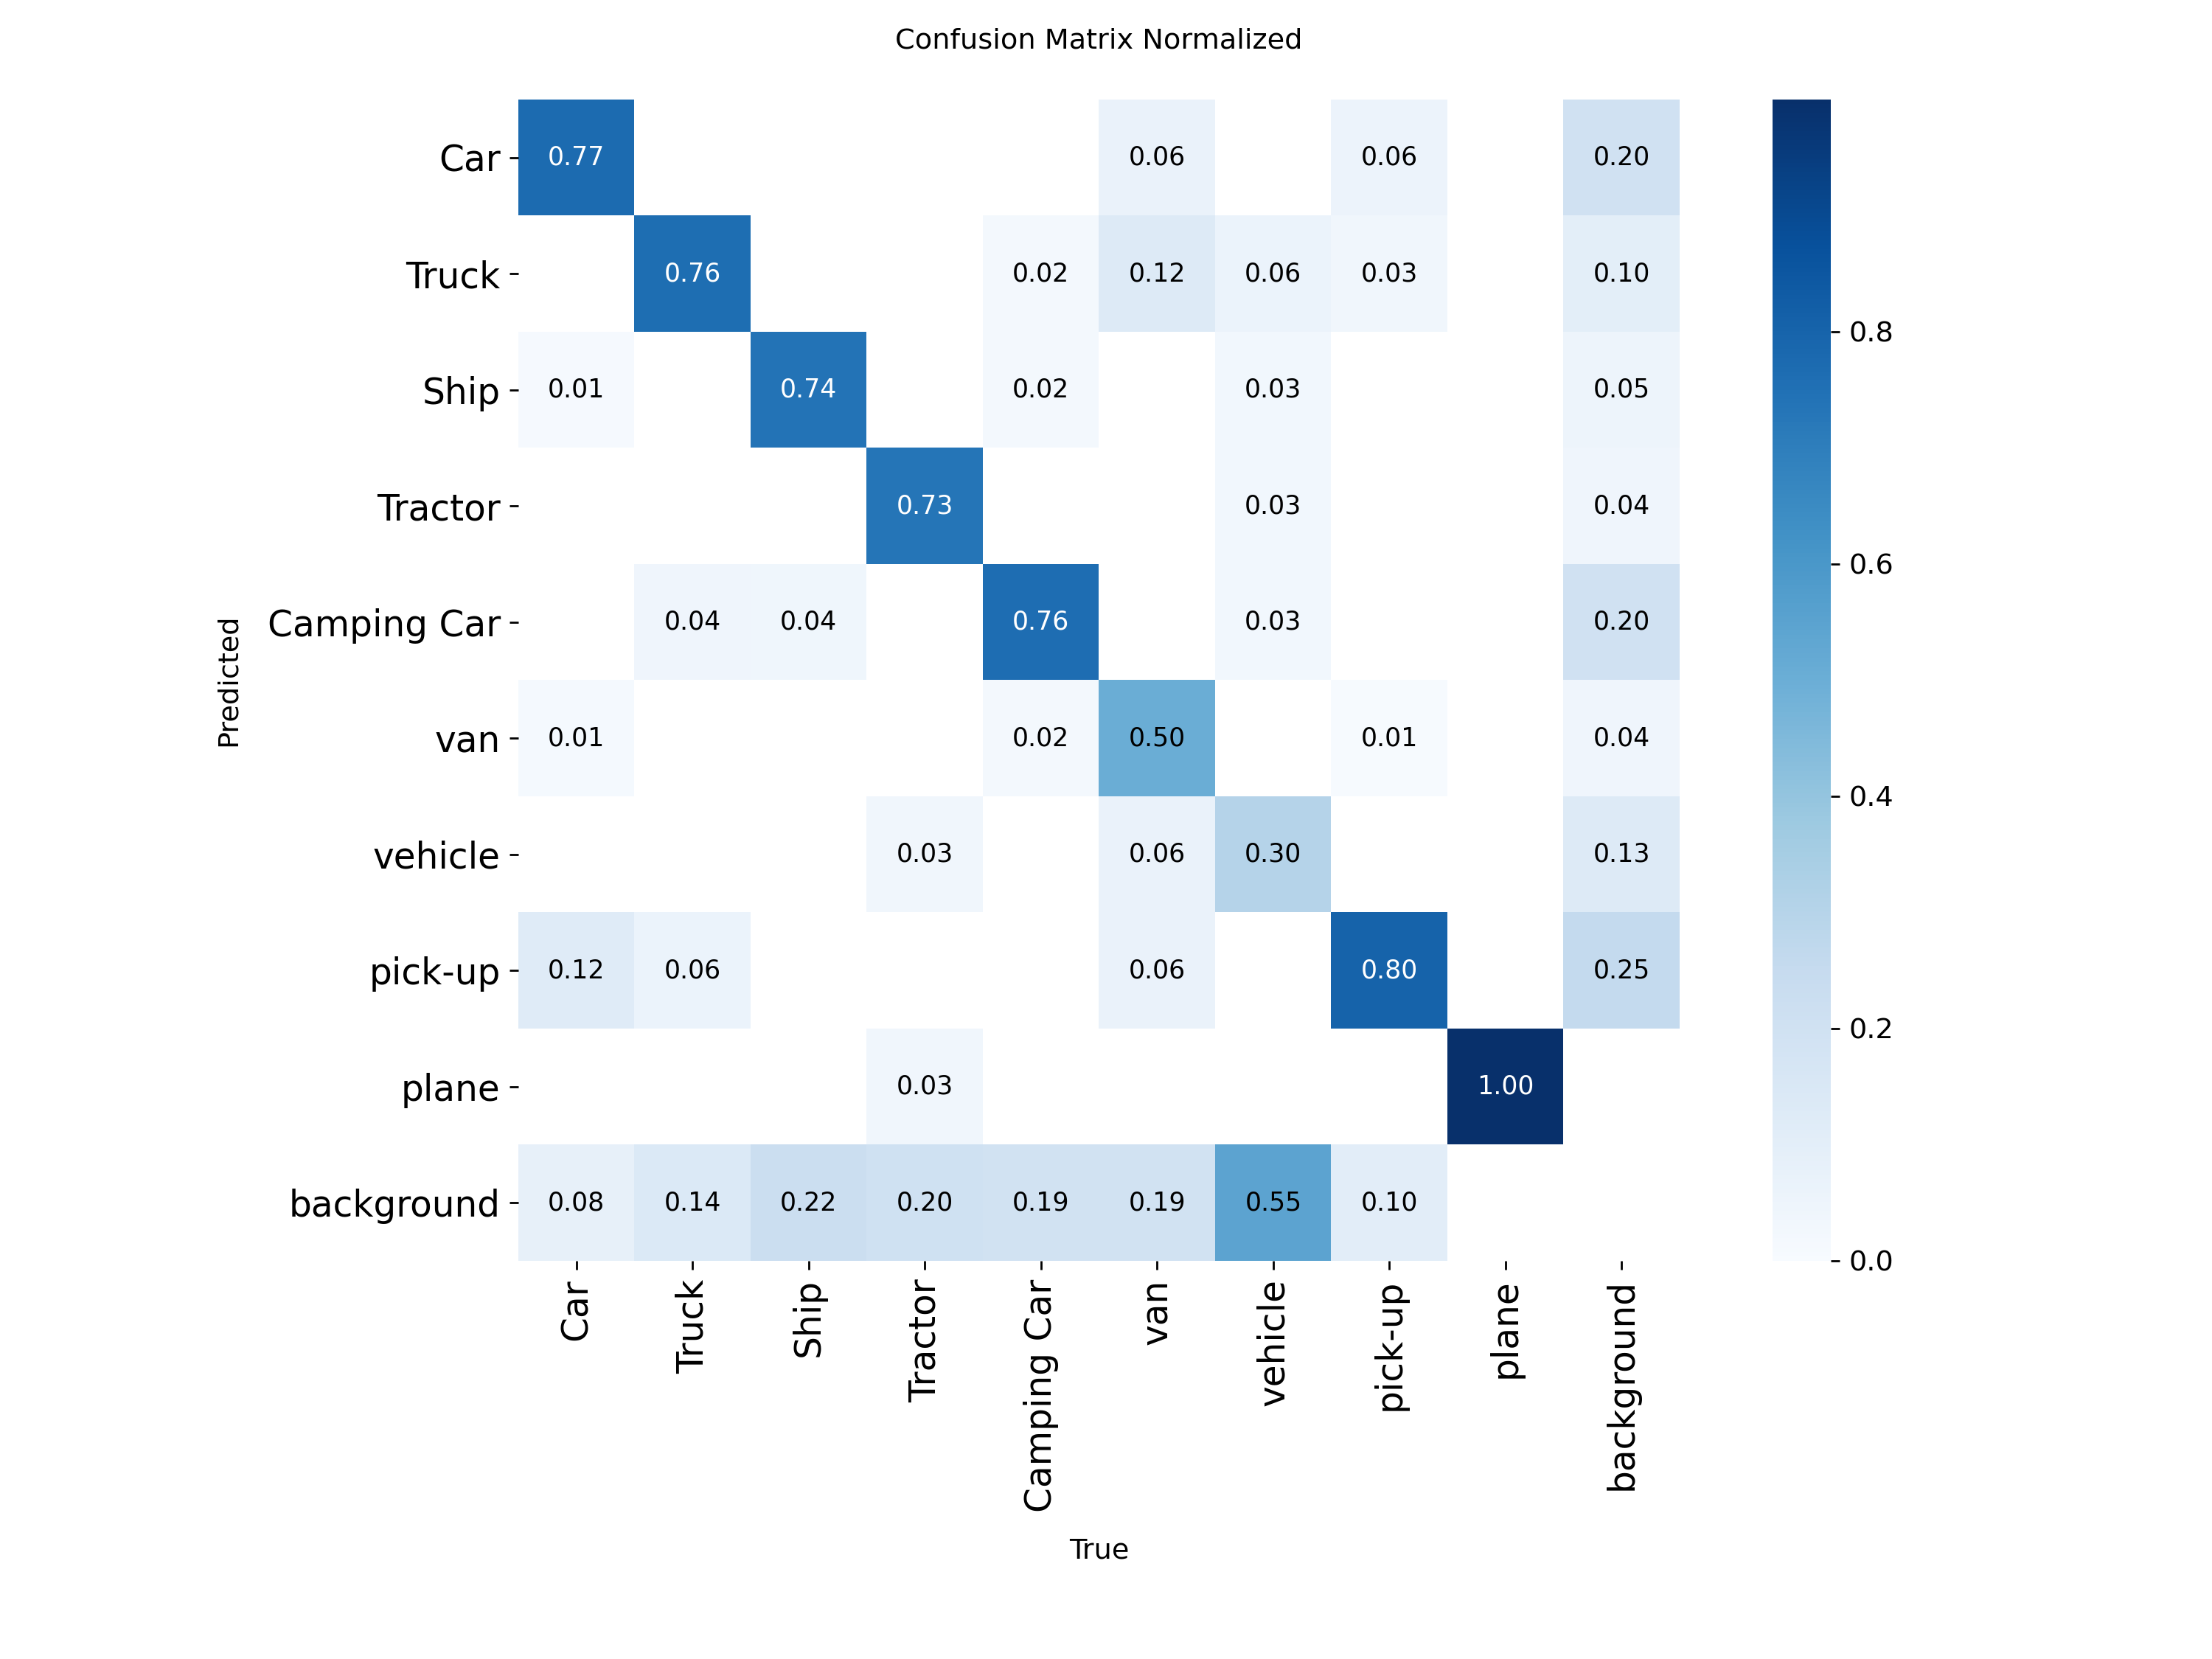
\includegraphics[width=\textwidth]{images/confusion_matrices/irgb_F4_confusion_matrix_normalized.png} % Bildpfad zum zweiten Bild
        \caption{ir-g-b} % Unterschrift für das zweite Bild
        \label{fig:cm_irgb} % Label für Referenzierung von Bild 2
    \end{subfigure}
    \caption{Comparison of Confusion Matrices between r-g-b-ir und ir-g-b for Fold 4} % Gemeinsame Unterschrift für beide Bilder
    \label{fig:combined_maps} % Label für die gesamte Figure-Umgebung
\end{figure}